\documentclass[10pt,twocolumn]{article}

\usepackage[UTF8,fontset=none]{ctex}
\setCJKmainfont[AutoFakeBold=2.5,AutoFakeSlant=0.18]{Songti SC}
\setCJKsansfont[AutoFakeBold=2.5]{Hiragino Sans GB}
\setCJKmonofont{Hiragino Sans GB}
\usepackage[a4paper,left=1.65cm,right=1.65cm,top=1.55cm,bottom=1.75cm]{geometry}
\usepackage{graphicx}
\usepackage{amsmath,amssymb,booktabs}
\usepackage[round,authoryear]{natbib}
\usepackage{caption}
\usepackage{subcaption}
\usepackage[unicode,colorlinks=true,linkcolor=black,citecolor=blue!55!black,urlcolor=blue!65!black]{hyperref}
\usepackage{xcolor}

\setlength{\columnsep}{0.62cm}
\setlength{\parindent}{2em}
\setlength{\parskip}{0.12em}
\renewcommand{\baselinestretch}{1.07}
\captionsetup{font=small,labelfont=bf}
\sloppy

\title{达尔文哥德尔机器：自我改进智能体的开放式演化}
\author{Jenny Zhang\textsuperscript{*,1,2}\quad
Shengran Hu\textsuperscript{*,1,2,3}\quad
Cong Lu\textsuperscript{1,2,3}\quad
Robert Lange\textsuperscript{\dag,3}\quad
Jeff Clune\textsuperscript{\dag,1,2,4}\\[0.5em]
\small \textsuperscript{1}英属哥伦比亚大学\quad
\textsuperscript{2}Vector Institute\quad
\textsuperscript{3}Sakana AI\quad
\textsuperscript{4}Canada CIFAR AI Chair\\
\footnotesize \texttt{\{jennyzzt,srhu,conglu\}@cs.ubc.ca},
\texttt{robert@sakana.ai}, \texttt{jeff.clune@ubc.ca}\\[-0.2em]
\footnotesize \textsuperscript{*}共同第一作者\quad \textsuperscript{\dag}共同资深作者}
\date{}

\begin{document}
\maketitle

\begin{abstract}
当今大多数 AI 系统受限于由人类设计的固定架构，无法自主且持续地改进自身。与之相对，科学方法是一个累积而开放的体系，每项创新都建立在既有成果之上，并使未来的发现成为可能。人们日益期待，当前依靠人工推进 AI 的过程本身也能实现自动化。如果能够安全地做到这一点，自动化将加速 AI 的发展，使我们更早获得其益处。这一前景提出了一个问题：AI 系统如何在不断提高相关问题求解能力的同时，无止境地改进自身？元学习能够自动发现新算法，但它受限于一阶改进，也受限于人类对适当搜索空间的设计。哥德尔机器~\citep{schmidhuber2007godel} 提出了一种理论上的替代方案，即让自我改进 AI 反复以可证明有益的方式修改自身。然而在实践中，要证明大多数改动具有净收益是不可能的。本文提出达尔文哥德尔机器（Darwin G\"odel Machine，DGM）：一种新的自我改进系统，它迭代修改自身代码，因此也改进修改自身代码库的能力，并使用编程基准对每项改动进行经验验证。DGM 受到达尔文演化和开放式研究的启发，持续扩充由已生成编程智能体构成的档案库。它从档案库中采样智能体，令这些智能体通过自我修改产生新颖而有趣的自身版本。这种开放式探索形成一棵不断生长的树，其中包含多样且高质量的智能体，并允许系统并行探索搜索空间中的多条不同路径。实验表明，DGM 能够自动提升编程能力，例如发现更好的代码编辑工具、长上下文窗口管理方法和同行评审机制，使 SWE-bench 上的性能从 20.0\% 提高到 50.0\%，Polyglot 上的性能从 14.2\% 提高到 30.7\%。此外，DGM 显著优于不具备自我改进或开放式探索的基线。所有实验都采用了沙箱和人工监督等安全措施。总体而言，DGM 朝着自我改进 AI 迈出了重要一步：它能够沿着通往无尽创新的展开路径，自行收集可供后续利用的垫脚石。全部代码已开源于 \href{https://github.com/jennyzzt/dgm}{https://github.com/jennyzzt/dgm}。
\end{abstract}

\section{引言}
\label{sec:intro}

科学进步具有累积性和开放性，每一次突破都建立在无数先前见解之上。同样，我们最先进的 AI 系统也源自一条漫长的创新谱系。例如，作为当代大语言模型（LLM）~\citep{brown2020language} 骨干的 Transformer~\citep{vaswani2017attention} 并非凭空出现，而是建立在多年既有创新之上，其中包括循环神经网络~\citep{linnainmaa1970representation,amari1972learning,hopfield1982neural,rumelhart1985learning} 和注意力机制~\citep{schmidhuber1990learning,bahdanau2015neural,kim2017structured,parikh2016decomposable}。然而，当今大多数 AI 系统仍受人类设计的固定架构约束，只能在预定义边界内学习，不能自主改写自己的源代码来实现自我改进。因此，AI 开发的每一次进展仍高度依赖人工干预，进步速度也随之受到牵制。本文考察一种引人关注的可能性：安全地自动搜索越来越好的 AI。我们可以设想这样一种 AI 系统，它像科学发现本身一样成为推动自身进步的引擎，在既有成果上继续构建，递归地改进自身，并把自己推向更高级的能力。

\begin{figure*}[t]
  \centering
  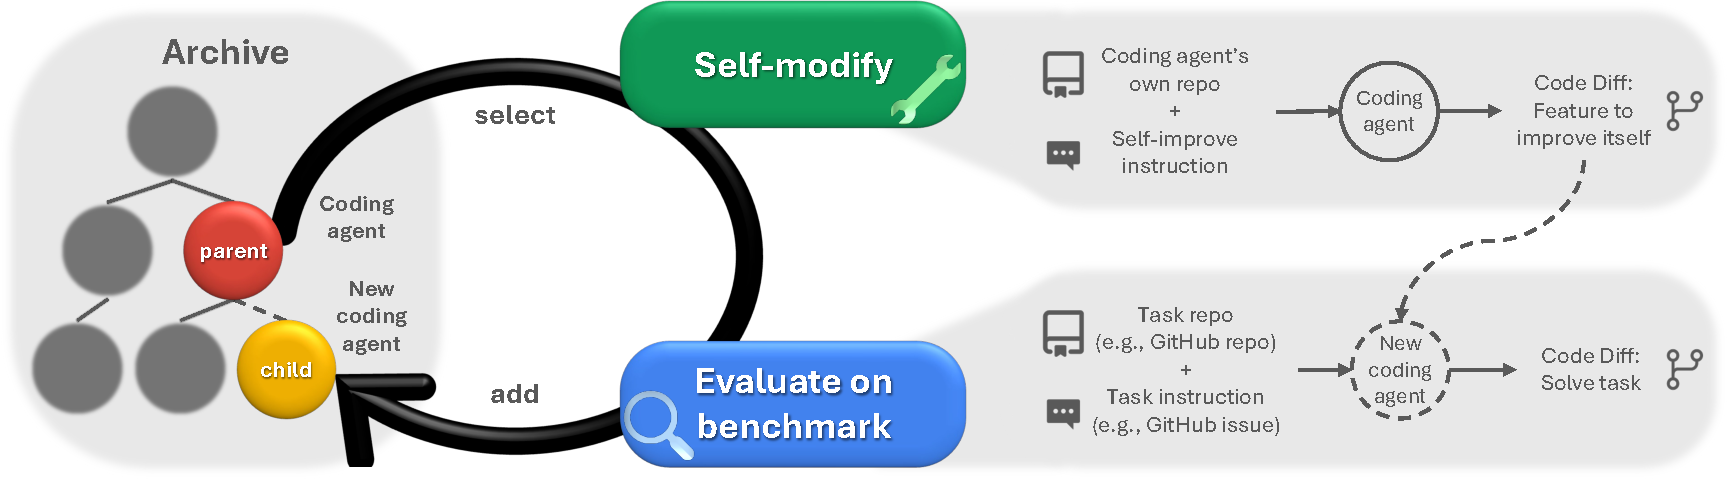
\includegraphics[width=0.93\textwidth]{figures/conceptual.pdf}
  \caption{\textbf{达尔文哥德尔机器。}DGM 在自我修改与下游任务评测之间交替，迭代构建一个不断扩大的智能体档案库。档案库中的智能体通过开放式探索被选中并进行自我修改。}
  \label{fig:conceptual}
\end{figure*}

\citet{schmidhuber2007godel} 提出了一类数学上严格、自指且能自我改进的问题求解器。它依靠形式化证明来论证代码重写的合理性，从而保证任何自我修改都可证明地有益。然而在实践中，如果不对系统施加强限制，就不可能形式化证明某项 AI 系统修改是否有益。例如，让基于 LLM 的编程智能体访问更多工具，例如代码搜索和测试运行器，看起来可能有益，但实际影响高度依赖模型训练和任务上下文。例如，针对一种环境优化的测试工具在其他环境中工作时反而可能使智能体困惑。我们不要求形式证明，而是在基准上对自我修改进行经验验证，使系统能够依据观测结果进行改进和探索。这一方法类似于生物演化：突变和适应不会被预先验证，而是先产生、再试验，最后由自然选择加以筛选。我们也从达尔文演化~\citep{darwin2023origin} 中获得启发，并研究维护一个既有智能体库、使其成为后续世代垫脚石的有效性。

本文提出\textbf{达尔文哥德尔机器（DGM）}，这是一种自指、自我改进的系统，它通过编写和修改自己的代码来成为更好的编程智能体。每次自我修改都要求 DGM 编辑自己的代码库。我们使用图灵完备的 Python，使 DGM 原则上具备构造任意可计算机器的潜力。我们的框架设想智能体能够重写自己的训练脚本，其中包括训练新的基础模型（FM）。但本文没有展示这一点，因为训练基础模型需要大量计算资源，还会引入显著的额外复杂度，我们将其留作未来工作。本文转而关注如何在冻结的预训练基础模型之上改进编程智能体的设计，例如工具使用和工作流。DGM 在自我修改阶段与评测阶段之间交替。在自我修改阶段，从档案库选出的编程智能体会生成经过修改的自身版本。在评测阶段，每个修改后的智能体都在编程基准上接受测试，以估计其编程能力，随后被加入档案库。DGM 通过这一循环改进自身能力，因而既更擅长解决编程任务，也更擅长实施未来的自我改进。这里的一项关键假设是，编程基准性能的提高意味着编程能力更强，进而意味着自我修改和自我改进能力更强。此外，DGM 从仅含一个智能体的档案库开始，并随时间持续积累所有生成的变体。为支持持续的自我改进，DGM 借鉴开放式研究~\citep{wang2019paired,fernandopromptbreeder,faldor2025omni}，积累多样化的垫脚石，也就是当前有趣但次优、却可能促成未来突破的解或特性。这种开放式探索鼓励系统发现超越即时性能收益的新颖且可能有用的自我修改。

我们在两个编程基准上给出结果：SWE-bench~\citep{jimenez2024swebench} 和 Polyglot~\citep{gauthier2024polyglot}。DGM 在 SWE-bench 上将自身性能从 20.0\% 自动提高到 50.0\%，在 Polyglot 上从 14.2\% 提高到 30.7\%。我们表明，自我改进能够带来持续进展：DGM 优于这样一种基线，即反复使用同一个基础智能体去修改并生成新智能体，却不让修改者自身得到改进。我们还表明，开放式探索以及保留全部既有智能体的档案库会促成更好的编程智能体。DGM 优于没有开放式探索的基线；该基线不积累有趣且不同的垫脚石，总是从自身最新版本继续构建。总体而言，DGM 朝着能够基于自身既有创新递归改进的 AI 系统迈出了一步。为了确保负责任的实验，我们广泛考虑并讨论了安全问题，其中包括沙箱和自我修改的可追溯性，见第~\ref{sec:safety} 节。通过推进安全、自指、自我改进模型的可能性，DGM 使我们更接近这样一种 AI：它不只是学习，还像科学本身一样沿着开放且自我加速的轨迹演化。

\section{相关工作}
\label{sec:related}

\textbf{开放式性。}
要推动不受限的创新，一个重大挑战是设计能够持续产生新颖且可学习产物的开放式 AI 系统~\citep{stanley2017open}。\citet{hughes2024open} 将开放式性刻画为：一个系统能够生成一系列从观察者视角看既新颖又可学习的产物。核心困难在于如何组织并探索巨大的搜索空间，从而持续生成对人类有趣的产物~\citep{clune2019ai,jiang2023general}。早期进展借助质量-多样性算法、目标导向探索、内在动机和学习进展框架~\citep{pugh2016quality,ecoffet2019go,lehman2011novelty,oudeyer2007intrinsic}；近期进展则利用大规模基础模型作为人类兴趣的代理，并把它们用作能在不同领域生成和评估新行为的通用引擎~\citep{brown2020language,hu2025automated,zhang2024omni}。然而，这些方法仍未闭合自指的自我改进循环，也就是说，下游任务上的改进不会转化为更强的自我修改能力，也不会加速后续创新。我们的目标是模拟科学技术的加速过程，其中新工具和新发现会催生更多发现。自然演化的轨迹不仅趋向更高复杂度，还趋向越来越强的可演化能力~\citep{dawkins2019evolution,gerhart2007theory,hendrikse2007evolvability}；我们要问的是，如何仿效这一轨迹？

\textbf{元学习基础模型智能体。}
许多基于基础模型的智能体都是手工设计的。常见构件包括提示工程~\citep{chen2023unleashing,schulhoff2024prompt}、思维链~\citep{wei2022chain,yao2023react,hu2023ThoughtCloning,guo2025deepseek,lightman2023let,muennighoff2025s1,zelikman2024quiet}、自我反思~\citep{shinn2023reflexion,yao2023react,madaan2303self}、多智能体辩论~\citep{zhuge2023mindstorms,liang2023encouraging,khan2024debating}、记忆~\citep{liu2023think,zhong2024memorybank,modarressi2023ret}、温度采样~\citep{zhu2024hot} 和检索增强生成~\citep{lewis2020retrieval}。人工组合这些组件，会使系统能力受限于人类设计者的才智。近期出现了若干元学习方法，它们利用基础模型自动优化提示~\citep{fernandopromptbreeder,meta2022human,khattab2023dspy,cheng2025trace,yuksekgonul2024textgrad,yuan2024evoagent} 并设计智能体模块~\citep{zhang2024aflow,zhou2024symbolic,yin2024g,zhugegptswarm,rosser2025agentbreeder,zhang2025multi,ye2025mas,gao2025flowreasoner,nie2025weak,su2025debflow,zhang2025gnns,niu2025flow}。智能体系统自动设计方法（Automated Design of Agentic Systems，ADAS）~\citep{hu2025automated} 使用一个固定的元智能体迭代生成下游智能体，在目标基准上评估它们，并吸收反馈以改进后续世代。与之不同，DGM 是一个既解决下游任务，也改进自身实现代码库的单一系统，因此不再需要固定的手工元智能体，并能够实现自指改进。

\textbf{自我改进 AI。}
早期研究者提出了多种自我改进的理论和概念方法~\citep{good1966speculations,schmidhuber1987evolutionary,schmidhuber2007godel}。自动自我改进的若干实践方法包括由神经网络权重参数化定义的系统~\citep{schmidhuber1993self,hall2007self,hobbhahn2025swebenchmini,kirsch2022self,irie2022modern,irie2025metalearning,lu2023arbitrary,havrilla2024glore}。\citet{metz2021training} 开发了一种基于梯度的优化器，使用群体式训练~\citep{jaderberg2017population} 的一个变体进行自指元训练。\citet{lange2023discovering} 将该方法扩展到无梯度学习。\citet{silver2017mastering} 使用自博弈持续演化智能体，并在国际象棋和围棋等高难度领域达到超人水平。与 DGM 更接近的是近期利用基础模型智能体进行自我改进的方法~\citep{yin2024g,robeyns2025self,hu2024self,zelikman2024self,huang2022large,singh2023beyond}。\citet{zelikman2024self} 使用元智能体生成下游智能体，再依据生成解所带来的元效用更新元智能体。\citet{yin2024g} 使用单一系统同时解决下游任务并递归修改自身。然而，下游任务或元效用并不总与自我改进所需的能力一致。在 DGM 中，下游任务的改进直接反映自我改进能力的增强，因此具备实现自我加速进展的潜力。与本文最相似的是 \citet{robeyns2025self} 的同期工作，其中同一个智能体也递归地解决编程问题并修改自身代码库。DGM 与该工作，以及 \citet{zelikman2024self,yin2024g} 的主要区别在于，DGM 具有开放式探索循环，鼓励超越即时性能收益的自我修改，从而避免停滞在次优状态。原文附录的补充相关工作还讨论了程序综合和达尔文演化。

\section{达尔文哥德尔机器}
\label{sec:methods}

哥德尔机器是一种理论设想：AI 搜索能够\emph{可证明地}改进自身的方法~\citep{schmidhuber2007godel}。本文提出达尔文哥德尔机器（DGM），尝试实现人们长期以来构造哥德尔机器的愿景。哥德尔机器要求从理论上\emph{证明}某项改动会改进系统，DGM 则放宽了这一不切实际的要求，转而要求实验给出\emph{经验证据}，表明所提议的新版本提升了性能。另外，由于 DGM 依赖改进的经验证据，它可能陷入潜在系统的巨大搜索空间，也就是全部可计算算法中的某个局部最优。为解决这一问题，DGM 在搜索期间维护已发现解的档案库，促进开放式探索，而不是只演化一个解。这一原则呼应达尔文演化~\citep{darwin2023origin}：从既有解的档案库中选择一个实体，对其加以修改，并在新实体有趣时将其保留~\citep{zhang2024omni,faldor2025omni,stanley2015greatness}。因此，我们将该算法称为达尔文哥德尔机器，见图~\ref{fig:conceptual}。

\textbf{编程智能体的自指自我改进。}
DGM 初始化时只有一个编程智能体，其进展通过编程基准评估。编程智能体被定义为一个由代码仓库实现、由冻结的预训练基础模型驱动、能够读写并执行代码的单一系统。当代码用通用的图灵完备语言表达，例如 Python，它就是构造和改进智能系统的强大媒介，因为它能够表示任何可计算过程。近期工作~\citep{hu2025automated,zhang2024aflow} 表明，可以通过元学习来改进这类智能体的设计，例如提示、工作流和工具，而这些设计都实现在代码仓库中。因此，我们把自我改进定义为一项编程任务，它修改智能体自身组件的设计，也就是修改自己的代码；这里不包括下一段所述的开放式探索过程。关键动机在于，经验证据必须同时反映系统的自我改进能力和下游任务求解能力。通过把 DGM 配置成编程智能体并测试其编程能力，观测到的改进不仅表明下游任务性能增强，也表明进一步自我改进的能力增强，因为自我改进从根本上就是一项修改编程智能体自身代码仓库的编程任务。

\textbf{基于群体的开放式探索。}
DGM 从一个初始编程智能体出发，构建包含所有已发现智能体的档案库。在每次迭代中，DGM 选择父智能体进行自我修改，并通过分支产生新智能体。父节点的选择概率大致正比于各智能体的性能分数，并反比于其具备代码库编辑能力的子节点数量，具体规则见原文附录“父节点选择”。这一规则偏好性能高但尚未得到充分探索的智能体，也就是现有子节点较少的智能体，因此既能利用表现强的智能体，又能探索有希望但采样较少的谱系。所有智能体都保留非零的选择概率，从而保证只要计算量充分，任何改进路径仍有可能被探索。

每个被选中的父智能体会分析自己的基准评测日志，提出下一项要实现的特性，再把该提议作为问题陈述交给自己执行，相关提示见原文附录“自我改进提示”。随后，父智能体把建议特性实现到自己的代码库中，产生新的编程智能体。每个新智能体都在选定的编程基准上接受定量评测，以估计其编程能力。只有能够成功构建并仍然能够编辑给定代码库的智能体才会被加入 DGM 档案库，因为只有它们能继续进行自我修改；其余智能体都会被丢弃。父节点选择、自我修改与评测的循环不断进行，逐步扩大解的档案库。需要特别指出，档案中的解可以在被发现很久以后才成为带来改进的垫脚石，因此本文方法与爬山式智能体设计方法~\citep{robeyns2025self} 有实质区别。目前，开放式探索过程，也就是档案维护和父节点选择，仍是固定的，不能被 DGM 修改；我们将其留作未来工作。原文附录给出了 DGM 算法的伪代码。

\section{实验}
\label{sec:experiments}

第~\ref{sec:experiment-setup} 节介绍实验设置，其中包括用于初始化 DGM 的初始编程智能体。我们在 SWE-bench~\citep{jimenez2024swebench} 和 Polyglot~\citep{gauthier2024polyglot} 两个编程基准上开展实验，见第~\ref{sec:benchmarks} 节。对于每个基准，我们将 DGM 与两个基线比较：不使用自我改进智能体的 DGM，以及不使用开放式探索的 DGM，见第~\ref{sec:baselines} 节。在所有实验中，DGM 都优于这两个基线，表明自我改进机制和开放式探索对于持续提高性能不可或缺，见第~\ref{sec:results} 节。此外，我们还表明，DGM 发现的特性可以在模型、基准和任务之间迁移。

\subsection{实验设置}
\label{sec:experiment-setup}

DGM 由单个编程智能体初始化。该基础智能体以冻结的基础模型为核心，并添加工具使用能力~\citep{schick2023toolformer,anthropic_tool_use_2024}。基础模型在每一步自主决定采取何种动作，并使用它认为合适的工具。基础智能体可以访问两个工具：一个用于执行 Bash 命令的 Bash 工具，以及一个用于查看和编辑目录与完整文件的编辑工具，具体实现见原文附录“初始编程智能体”。智能体只接收一个输入提示，其中指定目标仓库的位置、问题陈述以及仓库的测试框架。我们有意保持基础智能体的轻量化，使其成为一个简单起点，以便清楚展示后续自我改进。DGM 运行 80 次迭代，每次迭代生成一个新智能体；SWE-bench 实验并行运行两次迭代，Polyglot 实验并行运行四次迭代。在自我修改期间，SWE-bench 和 Polyglot 实验中的编程智能体均由 Claude 3.5 Sonnet (New)~\citep{anthropic2024claude35sonnet} 驱动。在基准评测期间，SWE-bench 使用 Claude 3.5 Sonnet (New)，Polyglot 使用 o3-mini~\citep{openai2025o3mini}。基础模型的超参数见原文附录。

\subsection{基准}
\label{sec:benchmarks}

我们使用两个流行基准评估 DGM，这两个基准衡量编程任务的不同方面，可用于验证算法在多种使用场景中的有效性。SWE-bench 和 Polyglot 都评估 AI 智能体自动解决编程任务的能力。给定一个代码仓库和一条任务指令，智能体应修改仓库以完成任务。这两个基准均被广泛使用~\citep{zhang2024autocoderover,zhang2024rest,xia2024agentless,cao2024spider2,GoogleDeepMind2025GeminiThinking,aider2024}，都要求 AI 智能体浏览代码仓库，理解不同文件中函数之间的相互作用，并找出复杂代码中的细小错误。SWE-bench 只包含 Python 任务，而 Polyglot 包含多种编程语言的任务。另一个区别是，每个 SWE-bench 任务可能要求编辑多个文件；每个 Polyglot 任务则主要要求从头在单个文件中实现一个解，尽管智能体仍需检查其他文件才能理解应做何种修改，因此总体文件编辑次数较少。

\textbf{SWE-bench。}
为避免把计算资源浪费在不可解任务上，我们采用 SWE-bench Verified~\citep{openai2024sweverified}，它是 SWE-bench~\citep{jimenez2024swebench} 经过人工筛选、所有任务均可解的子集。除非另有说明，本文中的 SWE-bench 默认指 SWE-bench Verified 子集。

\textbf{Polyglot。}
Polyglot 包含 C++、Rust、Python 等多种编程语言的任务~\citep{gauthier2024polyglot}。SWE-bench 是最常用的编程基准之一，很可能已被纳入基础模型训练集；相比之下，Polyglot 更为小众，被纳入基础模型后训练数据的可能性更低。此外，Polyglot 主要由其开发者用于评估 Aider~\citep{aider2024}。这为我们提供了一个机会：把自动设计的智能体与社区中的代表性编程智能体比较；Aider 由人类开发者持续开发了一年多，并始终在 Polyglot 基准上测试。最后，Polyglot 还能检验 DGM 跨越 Python、泛化到多种编程语言的能力。我们遵循 Polyglot 排行榜的设置~\citep{gauthier2024polyglot}，但有一项关键差异：排行榜报告 pass@2，智能体可以查看一次真实测试的反馈；我们报告 pass@1，智能体从不查看真实测试结果。

由于在完整基准上评测成本很高，成本估算见原文附录，我们采用分阶段评测策略来估计编程智能体的性能。一般而言，当我们更确信某个编程智能体表现较强时，才会用更多任务评测它。首先，我们在一组 10 个任务上评测每个编程智能体，以检查其基本代码库编辑能力。只有仍能编辑代码的智能体，才能解决下游编程任务或继续自我修改。通过初始阶段的智能体随后会在扩展的 50 个任务上评测。对于 SWE-bench，任务依据 SWE-bench-verified-mini~\citep{hobbhahn2025swebenchmini} 选择；该集合被设计为完整基准的代表性样本，任务清单见原文附录。对于 Polyglot，任务是从完整基准中随机抽取的子集，任务清单同样见原文附录。由于所用 LLM 本身具有随机性，性能可能存在噪声。我们使用较小子集上的评测来估计总体有效性并找出最佳候选。在 SWE-bench 上，如果某个编程智能体在 60 任务子集上的成功率超过 40\%，这一启发式阈值根据预实验中的噪声设定，并且它位列档案库前两名，那么我们会用 200 个任务进一步评测它，即另加 140 个任务，以更准确地估计其真实编程能力。对于 Polyglot，如果某个编程智能体在 10 任务子集上的成功率超过 40\%，则在扩展的 50 任务子集上评测它。

\subsection{基线}
\label{sec:baselines}

为分离并评估 DGM 核心组件各自的贡献，我们将 DGM 与两个基线比较：不使用自我改进智能体的 DGM（\textbf{DGM w/o self-improve}），以及不使用开放式探索的 DGM（\textbf{DGM w/o open-ended exploration}）。DGM w/o self-improve 在本设置中复现 ADAS~\citep{hu2025automated} 的方法：负责修改编程智能体的元智能体在整个实验中保持为固定的基础智能体。该基线使我们能够评估迭代式自我改进在加速更好编程智能体演化中的作用。DGM w/o open-ended exploration 不使用档案库，总是对自身最近保存的版本进行自我修改。如果编程智能体在自我修改后失去编辑代码库所需的基本功能，它就不能继续修改自身，也不能解决任何编程任务。因此，DGM w/o open-ended exploration 会保留仍具有基本代码库编辑功能的最新自身版本。该基线使我们能够评估档案库以及开放式探索中已有充分文献支持的有益原则~\citep{clune2019ai,stanley2015greatness,zhang2024omni,fernandopromptbreeder,lee2020learning,samvelyan2024rainbow,colas2022autotelic} 对智能体演化的影响。两个基线的伪代码见原文附录。

除学习得到的基线外，我们还将 DGM 与手工设计的开源方案比较。对于 SWE-bench，我们采用经过核验的开源最新最佳方案，即 SWE-bench 团队能够复现其结果的方案，详见原文附录。对于 Polyglot，我们采用代表性智能体 Aider~\citep{aider2024}；它已开源，并被设计为支持多种编程语言和大型代码库编辑。为公平比较，我们在评测 DGM 所用的相同基准子集上测量任务解决比例。图~\ref{fig:dgm-comparisons} 中的水平虚线表示这些数值。

\subsection{结果}
\label{sec:results}

\begin{figure*}[t]
  \centering
  \begin{subfigure}[t]{0.48\textwidth}
    \centering
    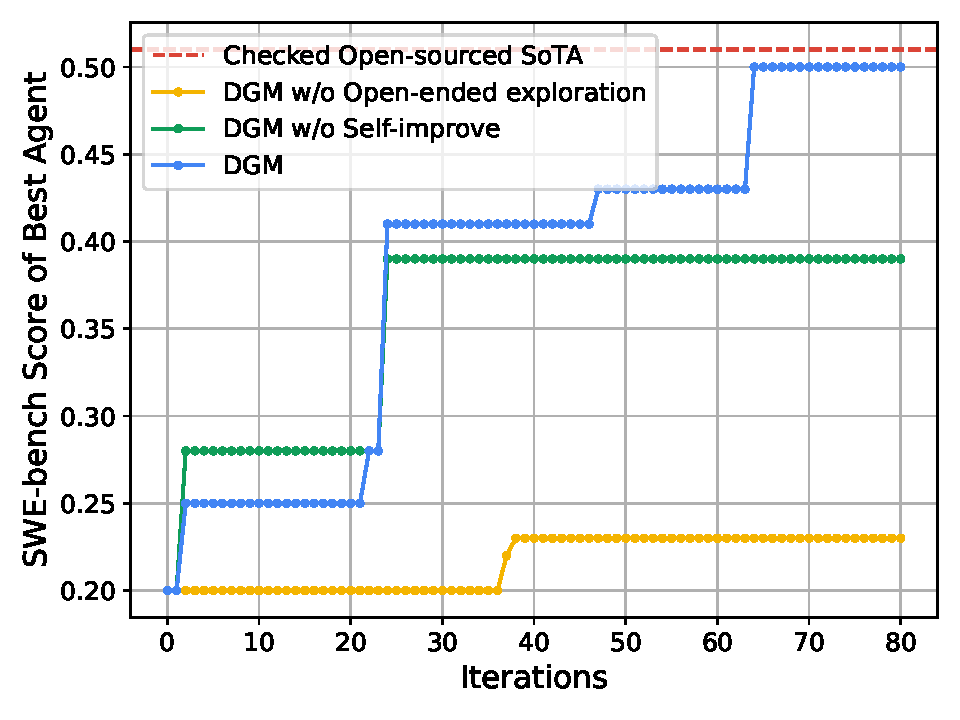
\includegraphics[width=\linewidth]{figures/dgm_comparisons.pdf}
  \end{subfigure}
  \hfill
  \begin{subfigure}[t]{0.48\textwidth}
    \centering
    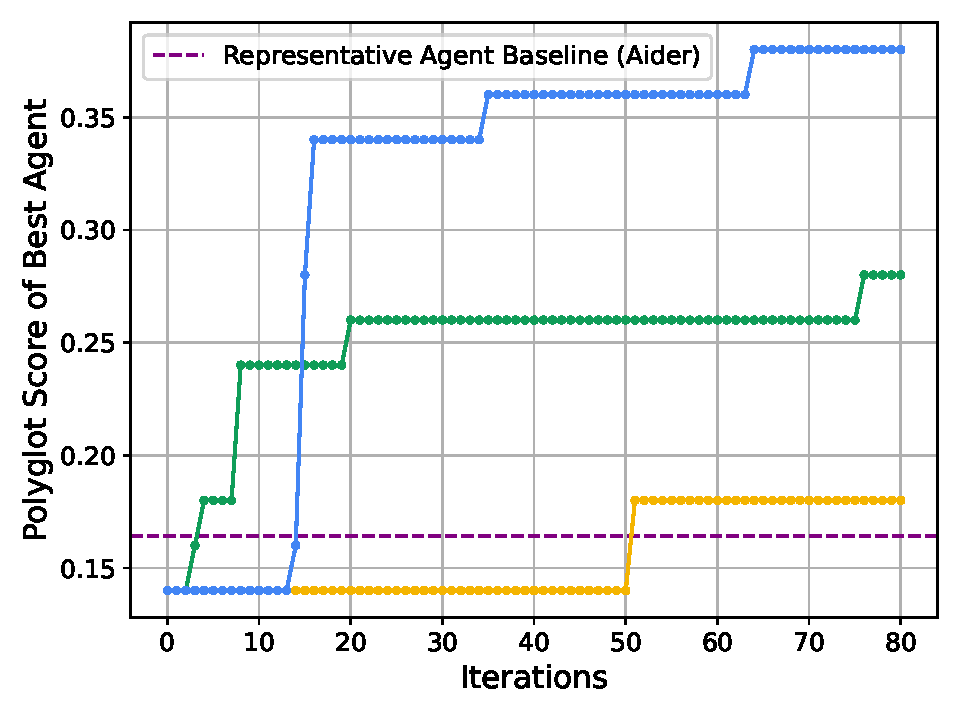
\includegraphics[width=\linewidth]{figures/dgm_comparisons_polyglot.pdf}
  \end{subfigure}
  \caption{\textbf{自我改进和开放式探索使 DGM 能够持续进展并提高性能。}DGM 自动发现越来越好的编程智能体，在左侧的 SWE-bench 和右侧的 Polyglot 上均取得更好表现。它优于缺少自我改进或开放式探索任一组件的基线，说明两者对于持续自我改进都不可或缺。这些分数来自第~\ref{sec:benchmarks} 节所述基准子集上的评测。}
  \label{fig:dgm-comparisons}
\end{figure*}

\begin{figure*}[t]
  \centering
  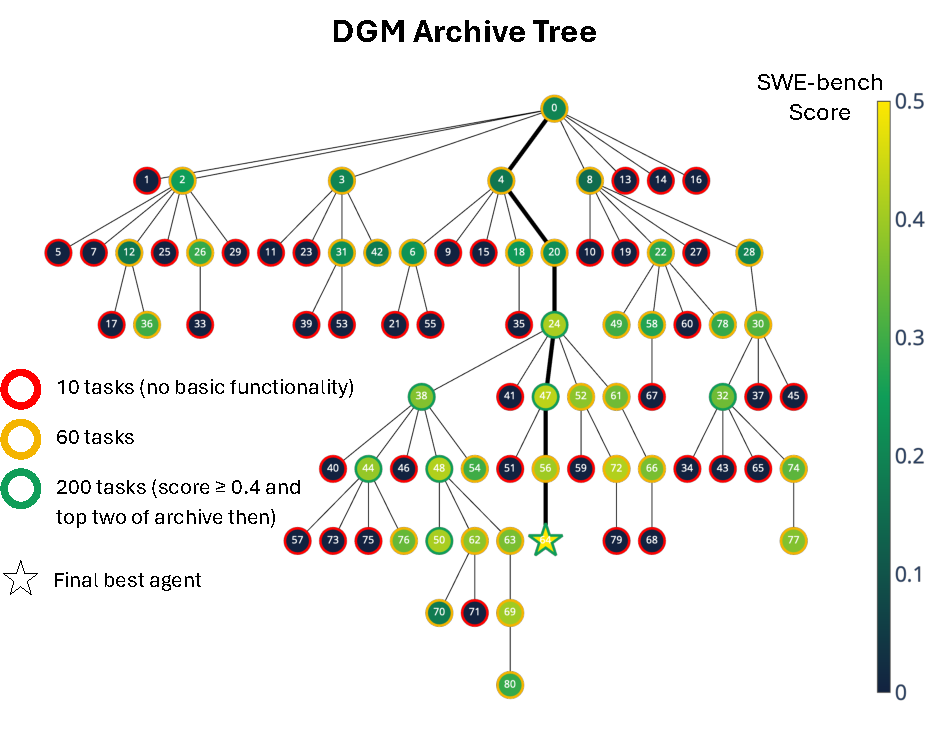
\includegraphics[width=0.47\textwidth]{figures/dgm_archive.pdf}
  \hfill
  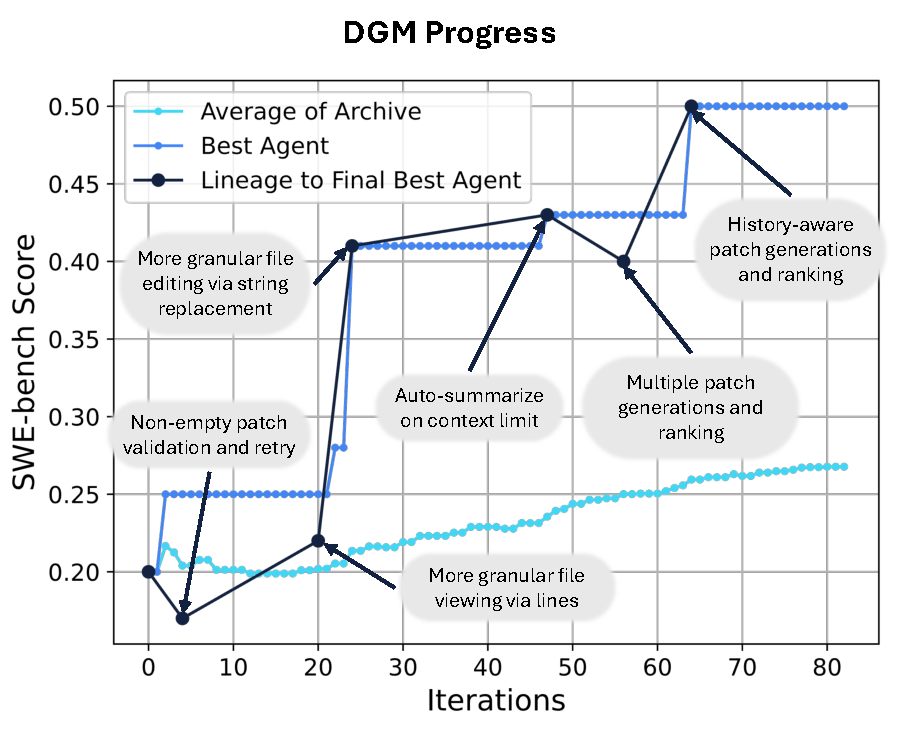
\includegraphics[width=0.47\textwidth]{figures/dgm_progress.pdf}
  \caption{\textbf{DGM 通过自动自我改进成为更好的编程智能体。}左图为 SWE-bench 上一次 DGM 运行期间生成的编程智能体档案库。每个节点代表一个编程智能体，节点 0 是基础智能体。节点颜色表示 SWE-bench 性能，即已解决任务的比例；边框颜色表示该智能体接受评测的任务数。边表示哪些智能体通过自我修改产生了后代。许多创新路径会经过性能较低的节点，而关键创新，例如节点 24，会引发建立在其上的大量后续创新；这两项性质都凸显开放式搜索的益处。右图为 DGM 在 SWE-bench 上的进展。浅蓝线表示所有具有基本代码库编辑功能的智能体的平均分，蓝线跟踪每次迭代时档案库内任一智能体达到的最高分，深色线表示最终最佳智能体及其前驱节点的谱系，其中包含两次性能下降。这说明开放式搜索的益处：它探索多样且有趣的垫脚石，而不是只从迄今发现的最佳解继续分支。}
  \label{fig:dgm-archive}
  \label{fig:dgm-progress}
\end{figure*}

DGM 运行 80 次迭代后，编程智能体在 SWE-bench 上的性能从 20.0\% 提高到 50.0\%，在 Polyglot 上从 14.0\% 提高到 38.0\%，见图~\ref{fig:dgm-comparisons}。由于 Polyglot 实验设置只在 50 个任务上评测 DGM，见第~\ref{sec:benchmarks} 节，我们又在完整 Polyglot 基准上评测基础智能体和 DGM 发现的最佳智能体，以更准确地估计改进幅度。在完整 Polyglot 基准上，DGM 将编程智能体的性能从 14.2\% 提高到 30.7\%。这表明 DGM 能够自动进行自我改进，创造出更好的编程智能体。此外，DGM 发现的最佳智能体在 SWE-bench 上与经过核验、开源且由人类设计的最新最佳方案性能相当，见图~\ref{fig:dgm-comparisons}。在 Polyglot 上，尽管 DGM 的基础智能体起点低于 Aider，它最终发现的智能体却大幅超过 Aider。DGM 发现的智能体在两个基准上都达到或超过手工智能体。SWE-bench 的最新最佳智能体和 Aider 都凝聚了大量人工设计工作，而 DGM 展示了一种未来可能性：这类才智可以自动化，并通过自指的持续自我改进循环不断演化。

DGM 会自动改进基础模型的工具和使用工作流，见图~\ref{fig:dgm-progress}。例如，DGM 改进了编辑工具，使其可以按行进行粒度更细的文件查看，也可以通过字符串替换进行更精确的文件编辑，而不必每次查看或替换整个文件。工作流方面的改进包括多次尝试解决任务，以及使用另一个基础模型评估并选择最佳解。其他工作流改进还包括在生成后续尝试时考虑先前尝试。原文附录完整列出了在 SWE-bench 和 Polyglot 上通往最终最佳智能体的所有修改。

因为开放式探索以非零概率允许系统从档案库中的任何智能体分支，DGM 能够走出具有欺骗性的性能低谷或高峰。例如，在 SWE-bench 实验的第 4 次和第 56 次迭代，智能体分数一度低于父节点，但 DGM 仍能沿该路径继续探索创新，并产生超过全部前驱的新智能体，见图~\ref{fig:dgm-progress}。此外，开放式探索允许系统尝试同一目标功能的不同实现。例如，目标都是提供粒度更细的编辑工具，但该特性的具体实现可以差异很大，并由此产生截然不同的性能，相关对照见原文附录。DGM 可以探索多种实现，找出最合适的方案，避免困在次优实现上。

DGM 在两个基准上都优于 DGM w/o self-improve 和 DGM w/o open-ended exploration，见图~\ref{fig:dgm-comparisons}。DGM w/o self-improve 不更新负责修改编程智能体的元智能体，因此虽然早期迭代能够改进智能体，收益却很快趋于停滞，补充曲线见原文附录。DGM w/o open-ended exploration 只保留最近的智能体，所以一次表现不佳的自我修改会使后续改进更难实现。

\begin{figure*}[t]
  \centering
  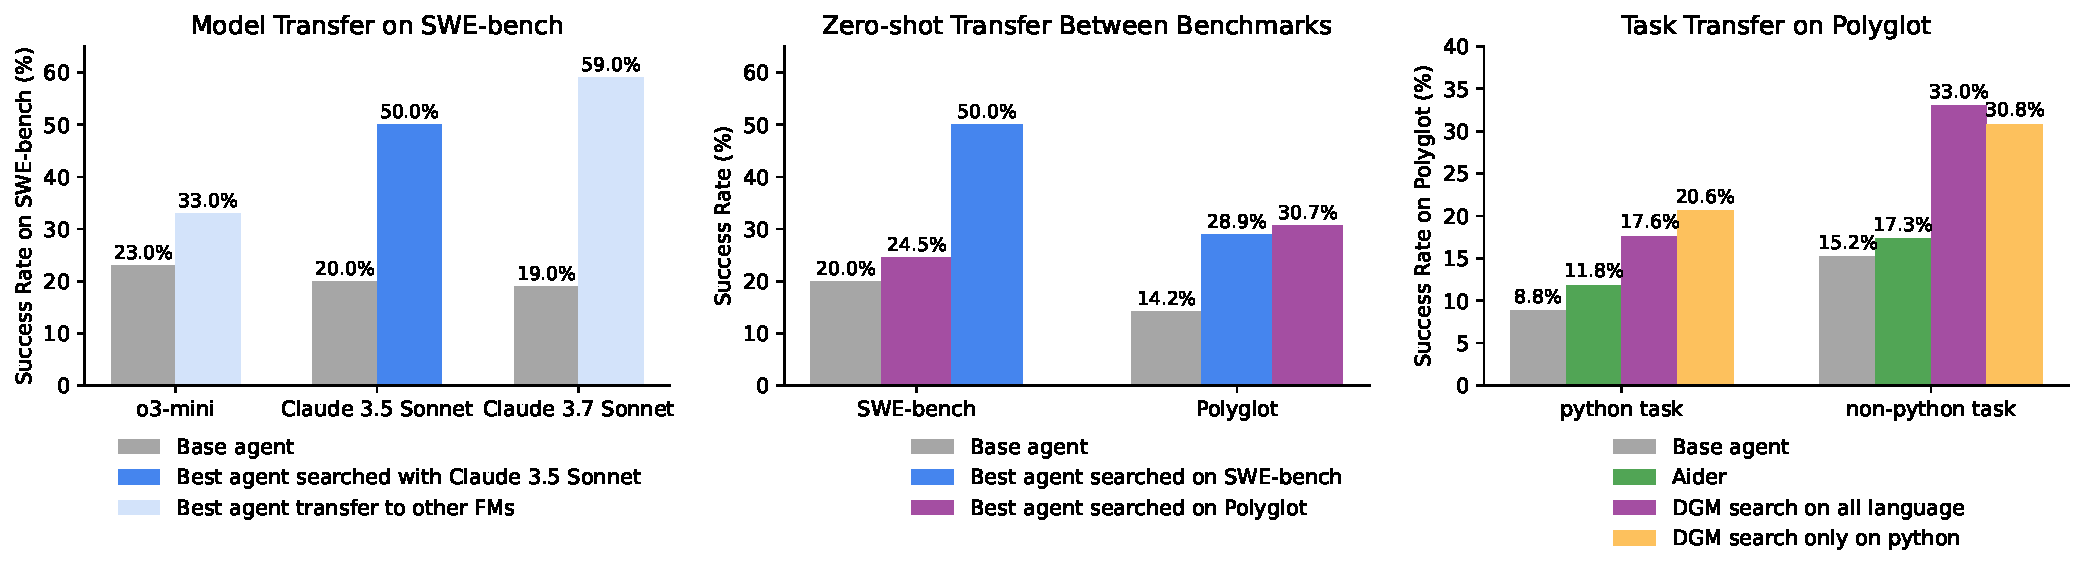
\includegraphics[width=0.94\textwidth]{figures/transfer_model_task.pdf}
  \caption{\textbf{模型、基准与任务之间的迁移。}DGM 所发现智能体的性能优势能够迁移到左侧的不同模型、中间的不同基准，以及右侧 Polyglot 中不同编程语言的任务，例如从 Python 任务迁移到 C++ 任务。}
  \label{fig:transfer-overview}
\end{figure*}

为评估 DGM 所带来改进的通用性，我们把基础智能体和一次 DGM 运行中发现的最佳智能体，换用优化期间未使用的基础模型进行测试。对于 SWE-bench，DGM 原先使用 Claude 3.5 Sonnet (New) 运行；迁移评测时，我们将基础模型换成 Claude 3.7 Sonnet~\citep{anthropic2025claude37} 或 o3-mini，并在 200 个任务上进行评测，见图~\ref{fig:transfer-overview} 左侧。使用 o3-mini 时，基础智能体取得 23.0\%，DGM 发现的智能体取得 33.0\%。使用 Claude 3.7 Sonnet 时，基础智能体取得 19.0\%，DGM 发现的智能体取得 59.5\%。这些结果表明，DGM 产生的改进可以跨基础模型泛化，而不是与运行时使用的特定基础模型紧密绑定。Polyglot 上的模型迁移结果见原文附录。

我们还研究了 DGM 所发现智能体在不同基准和编程语言之间的可迁移性。首先，我们把一个基准上 DGM 发现的最佳智能体，例如 SWE-bench 上的最佳智能体，拿到完全留出的另一个基准，例如 Polyglot 上评测，反向亦然，见图~\ref{fig:transfer-overview} 中间。在 SWE-bench 上演化出的最佳智能体在 Polyglot 上达到 28.9\%，而初始智能体的基线为 14.2\%。反过来，在 Polyglot 上演化出的最佳智能体在 SWE-bench 上达到 24.5\%，超过原始基线的 20.0\%。由于优化每个智能体时都从未访问另一个基准，这些评测是真正的留出测试。跨基准的一致性能增益支持我们的主张：DGM 的改进反映了通用技能的获得，而不是过拟合或利用特定基准的伪影。其次，我们让一个 DGM 版本只在 Polyglot 的 Python 任务上训练，再把发现的智能体迁移到其他语言的任务上。主要关注 Python 任务会略微提高 Python 任务性能，但与使用全部语言训练的 DGM 相比，会降低非 Python 任务性能，见图~\ref{fig:transfer-overview} 右侧。然而，在搜索期间从 Python 迁移到此前未见的其他语言后，该智能体仍能达到与全语言 DGM 相当的性能，并显著超过基础智能体和 Aider。这些结果说明所发现改进具有稳健性，不会过拟合某一种编程语言。原文附录还给出了更多结果。

\section{安全讨论}
\label{sec:safety}

DGM 这类能够自我改进的系统朝着更自主的 AI 开发迈出了一步，也与该领域长期以来构建能造福人类的强大 AI 这一目标一致~\citep{schmidhuber1987evolutionary,clune2019ai,markoff2016machines,lehman2023machine}。然而，自主修改自身代码的能力会带来独特的安全问题。如果修改只针对基准性能进行优化，即便提高了目标指标，也可能无意中引入漏洞或不符合人类意图的行为~\citep{bostrom2020ethical}。特别是，如果评测基准没有充分覆盖安全性和稳健性等全部期望属性，自我改进循环就可能在连续世代中放大不对齐。迭代式自我修改还可能产生越来越复杂、越来越难解释的内部逻辑，妨碍人类理解、监督和控制~\citep{sheth2025safety,anwar2024foundational,greenblatt2024alignment,ganguli2022red}。

认识到这些挑战后，DGM 当前实现和实验设置纳入了多项安全措施。所有智能体执行和自我修改过程都在隔离的沙箱环境中进行，限制其影响宿主系统的能力，从而降低非预期操作的风险。沙箱中的每次执行都受严格时间限制，以降低资源耗尽或行为无界的风险。当前自我改进只限于一个定义明确的范围：修改智能体自己的 Python 代码库，以提高特定编程基准上的性能，因此潜在修改的范围受到限制。此外，我们主动监控智能体性能和代码改动，DGM 档案库则提供了可供审查的可追溯修改谱系。在当前阶段，我们没有发现所生成智能体表现出有害或恶意行为的证据，自我修改主要集中在提高编程能力上。

另一方面，自我改进范式的一项重要潜在益处是，原则上可以把它导向安全性与可解释性本身的改进。我们进行了初步研究，考察如何在 AI 安全场景中部署 DGM，以开发针对基础模型幻觉的应对措施，详见原文附录。正如 DGM 学习改进编程能力一样，如果评测标准包含安全或透明性属性，它也可能发现并整合更好的内部安全措施，或通过自我修改获得更高透明度，例如纳入类似 Constitutional AI~\citep{bai2022constitutional} 的原则~\citep{rosser2025agentbreeder}。这表明一条有希望但充满挑战的路径：把自我改进变成构建更可信 AI 系统的工具。后续研究也可以探索从一开始就把 Constitutional AI 编织进系统；难点在于如何激励系统持续保留这些指令，一种值得探索的方案是设置系统中不可修改的部分，使其能够在其余部分停止时进行评估。

在前沿基础模型能力仍有限、且沙箱等缓解措施有效的条件下，DGM 展示了自我改进 AI 的潜力，同时仍运行在安全的研究边界内。原文附录进一步讨论了更广泛的安全不确定性。我们主动加入本节安全讨论，是为了提醒人们注意自我改进 AI 系统正在出现的前景及其相关安全影响，尤其考虑到这些系统的能力不可避免地会继续增强~\citep{yudkowsky2008artificial,bostrom2002a,ecoffet2020open,bengio2024managing,clune2019ai}。因此，我们主张继续研究 AI 生成算法~\citep{clune2019ai} 与自我改进系统如何安全且有益地演化。

\section{结论与局限}
\label{sec:conclusion}

本文提出达尔文哥德尔机器（DGM）。据作者所知，它是首个由基础模型驱动、具有开放式探索的自我改进系统，并且评测基准上的进展能够直接转化为更强的自我改进能力。我们展示了对更好工具和基础模型系统的自动发现，并由此在 SWE-bench 和 Polyglot 两个基准上获得更好性能。通过自我改进和开放式探索，DGM 的性能持续提高，使我们向自我加速、自我改进的 AI 系统又迈进一步。

我们表明，DGM 能够自主达到与公开可用方案相当的性能。但它仍落后于闭源的 SWE-bench 最新最佳方案。一个开放问题是，更长时间运行 DGM 是否会持续带来性能提升，并最终超过闭源方案。这些闭源方案通常依赖技术高超的专家团队精心手工设计的方法。由于基础模型尚未达到这类专家的能力，例如推理能力，DGM 当前需要大量计算才能发现改进。第~\ref{sec:experiments} 节所述的一次 SWE-bench DGM 运行大约需要两周，并产生高额 API 成本，成本估算见原文附录。我们推测，进一步进展需要更高效地利用计算资源，并发展更好的推理能力。

这一版 DGM 主要由基础模型驱动，因此天然受底层基础模型能力限制。一个令人期待的未来方向，是把自我修改从提示或基础模型工作流扩展到计算量更大的方法，例如重写自己的训练脚本以更新基础模型本身。当前 DGM 聚焦编程，但 AI 系统正在计算机视觉、创意写作等广泛领域得到应用。另一项有希望的扩展，是开发能够在编程以外领域改进自身的自我改进 AI 系统。本文的一项关键假设是，编程基准能很好地反映智能体的自我改进能力，因为自我修改任务要求智能体修改自己的代码库。然而，也可以设想一种替代方法，让目标任务分布共同演化~\citep{faldor2025omni,wang2023robogen}，从而摆脱把自我改进绑定在单一目标上的限制，更接近真正的开放式过程。原文附录给出了更多潜在未来方向。随着我们继续探索这项强大技术，也必须始终把第~\ref{sec:safety} 节所述安全问题置于核心位置。

总之，DGM 朝着通过能够编辑自身代码库的自我改进系统实现 AI 开发自动化迈出了重要一步。当前计算和推理能力的局限仍制约其全部潜力，但基础模型和基础设施的持续进步可能释放更强大、更通用的自我改进。只要审慎处理安全问题，见第~\ref{sec:safety} 节，自我改进 AI 系统和 AI 生成算法~\citep{clune2019ai} 的未来就具有巨大潜力：它们可以开放式地演化 AI，在追求与人类价值一致的更强能力时不断重写或重新训练自身。

\section*{伦理声明}

作者确认本研究符合 ICLR 伦理准则。本工作仅在一个受限情境中研究自我改进 AI 系统，即在标准编程基准上评测的代码编辑智能体。研究不涉及人类受试者，也未收集或处理任何个人身份信息，因此无需机构审查委员会批准。

\textbf{安全与滥用。}
如果允许自我修改系统不受约束地行动，或者优化过程无意中引入不安全行为，这类系统可能带来安全风险。为降低风险，实验中的所有智能体都运行在隔离沙箱中，具有严格的资源和时间限制；智能体只能进行有限的网络访问，也不能修改宿主环境。自我改进范围被限制在智能体自身的 Python 代码库和评测工具上。作者维护了完整且可审计的代码改动与评测谱系，也就是档案库，从而支持回滚和事后分析。作者没有在真实开发环境中部署所发现的智能体。发布代码、提示和评测产物时，任何授予高级系统访问权限的组件都将被排除，并将提供默认沙箱、安全护栏和清晰的预期用途文档。

\textbf{双重用途、下游影响与局限。}
能力更强的自主编程智能体可能具有双重用途，例如既能帮助维护软件，也可能在误用时帮助制作有害代码。作者认为，本研究的益处，例如推进可控、可审计的自我改进方法并展示实际安全措施，超过其风险。尽管如此，作者明确反对在安全敏感场景或无沙箱条件下部署，并在第~\ref{sec:safety} 节给出具体安全建议。只关注基准优化的实验可能无法覆盖稳健性、可解释性或更广泛社会价值等全部期望属性。因此，作者把基准收益视为通用 AI 开发的必要但不充分指标，并讨论了如何把安全、推理等其他目标纳入优化循环。

\textbf{数据治理、知识产权与许可。}
实验使用 SWE-bench Verified 和 Polyglot，两者由开源仓库和任务构成。据作者所知，研究遵守了数据集许可与使用条款，没有引入或分发专有代码。基础模型通过提供商 API 访问，并遵守其服务条款；研究既未提交敏感数据，也未尝试规避使用政策。随论文发布的日志将清除 API 密钥和任何偶然出现的敏感字符串。

\textbf{偏见、公平与平等。}
尽管研究领域是软件代码而不是以人为中心的文本，基础模型行为仍可能反映偏见，例如偏好某些语言或生态系统；训练数据中工具表示更充分的社区也可能获得不均衡的益处。作者通过在 Polyglot 的多种语言上评测并报告跨基准迁移，在一定程度上处理这一问题。未来工作应增加针对偏置失效模式的诊断，并纳入范围更广、由社区驱动的任务集。

\textbf{利益冲突与资助。}
没有作者在本文评测其性能的产品中拥有经济利益。除提供薪酬或常规研究支持外，资助者和雇主没有影响实验设计、分析或发表决定。任何外部计算资源或 API 额度均在原文附录中致谢。

\section*{可复现性声明}

作者将开源全部代码和完整智能体日志，其中包括自我修改的完整档案谱系，例如差异、提示和配置，以及评测工具。为支持精确复现，论文给出了以下内容：第~\ref{sec:methods} 节及原文附录中的算法细节与伪代码；原文附录中的父节点选择和开放式探索设置；基础模型选择与超参数；SWE-bench 和 Polyglot 的基准任务子集；第~\ref{sec:benchmarks} 节中的分阶段评测协议与脚本；最佳智能体的实现和差异；以及计算与成本估算。发布的代码仓库将包含环境规范，以及复现全部结果、图和表的脚本。

\subsubsection*{致谢}
本研究得到 Vector Institute、Canada CIFAR AI Chairs 计划、Schmidt Futures 资助、NSERC Discovery Grant 以及 Rafael Cosman 慷慨捐赠的支持。用于准备本研究的部分资源由安大略省、加拿大政府通过 CIFAR，以及赞助 Vector Institute 的公司提供，合作伙伴名单见 \url{https://vectorinstitute.ai/partnerships/current-partners/}。本文材料中表达的任何观点、发现、结论或建议均属于作者，不一定代表资助方立场。作者还感谢 Aaron Dharna、Ben Norman、C\'edric Colas、Sam Devlin 和 Shyam Sudhakaran 富有洞见的讨论与反馈。

\bibliographystyle{iclr2026_conference}
\bibliography{main}

\end{document}
